
\documentclass{article}
\usepackage[a4paper, total={6in, 8in}]{geometry}
\usepackage[utf8]{inputenc}
\usepackage{graphicx}
\usepackage{caption}
\usepackage{subcaption}
\usepackage[backend=biber, style=numeric, sortcites=true, sorting=none]{biblatex}
\addbibresource{references.bib}

\usepackage{multicol}
\usepackage{wrapfig}
\usepackage{latexsym}
\usepackage{lipsum}
\usepackage{float}           
\usepackage{amsmath}

\title{Thesis}
\author{Michael Fried }
\date{May 2019}

\begin{document}

\maketitle

\section{Introduction}
Optical Fibre introduction

Metal Semiconductor Junctions 
    Silicide Contacts
    Al Contacts
    oxide layers
    

    
CV measurements 

Lithography

Deposition

Sem and EDS
\section{Photolithography}
Photolithography is a microfabrication technique that allows for the patterning of 

\section{Four Point Probe Measurements}

\section{Electron Microscopy and Energy Despersive Spectroscopy}

\section{Polishing}

\section{mibots}
An alternative to the Lithographic techniques described, is direct probing of the sample using micro manipulators. Remina Techinology Mibots are micro manipulators with tungsten probes capable of electrical probing. The positioning precision is in the nm range making them capable of probing the smallest cores. Direct probing has the advantage of eliminating the challenges associated with lithography, including the need to bridge an cracking in the glass fiber and any relief profile and possible chipping at the glass epoxy interface. Problems with metal adhesion to the three different materials (glass,epoxy,core) are substrate is also eliminated. While work has been done to use micromanipulators to characterize semiconductor fibers \cite{Engel2016DirectPhotosynthesis} past experience in our group has found that reliable electrical contact is difficult to achieve. Ohmic contacts of the manipulators requires sufficient force (look up here). By defining contacts only on the core of the fiber, we hope to negate the problems encountered in the past and validate our current results. 

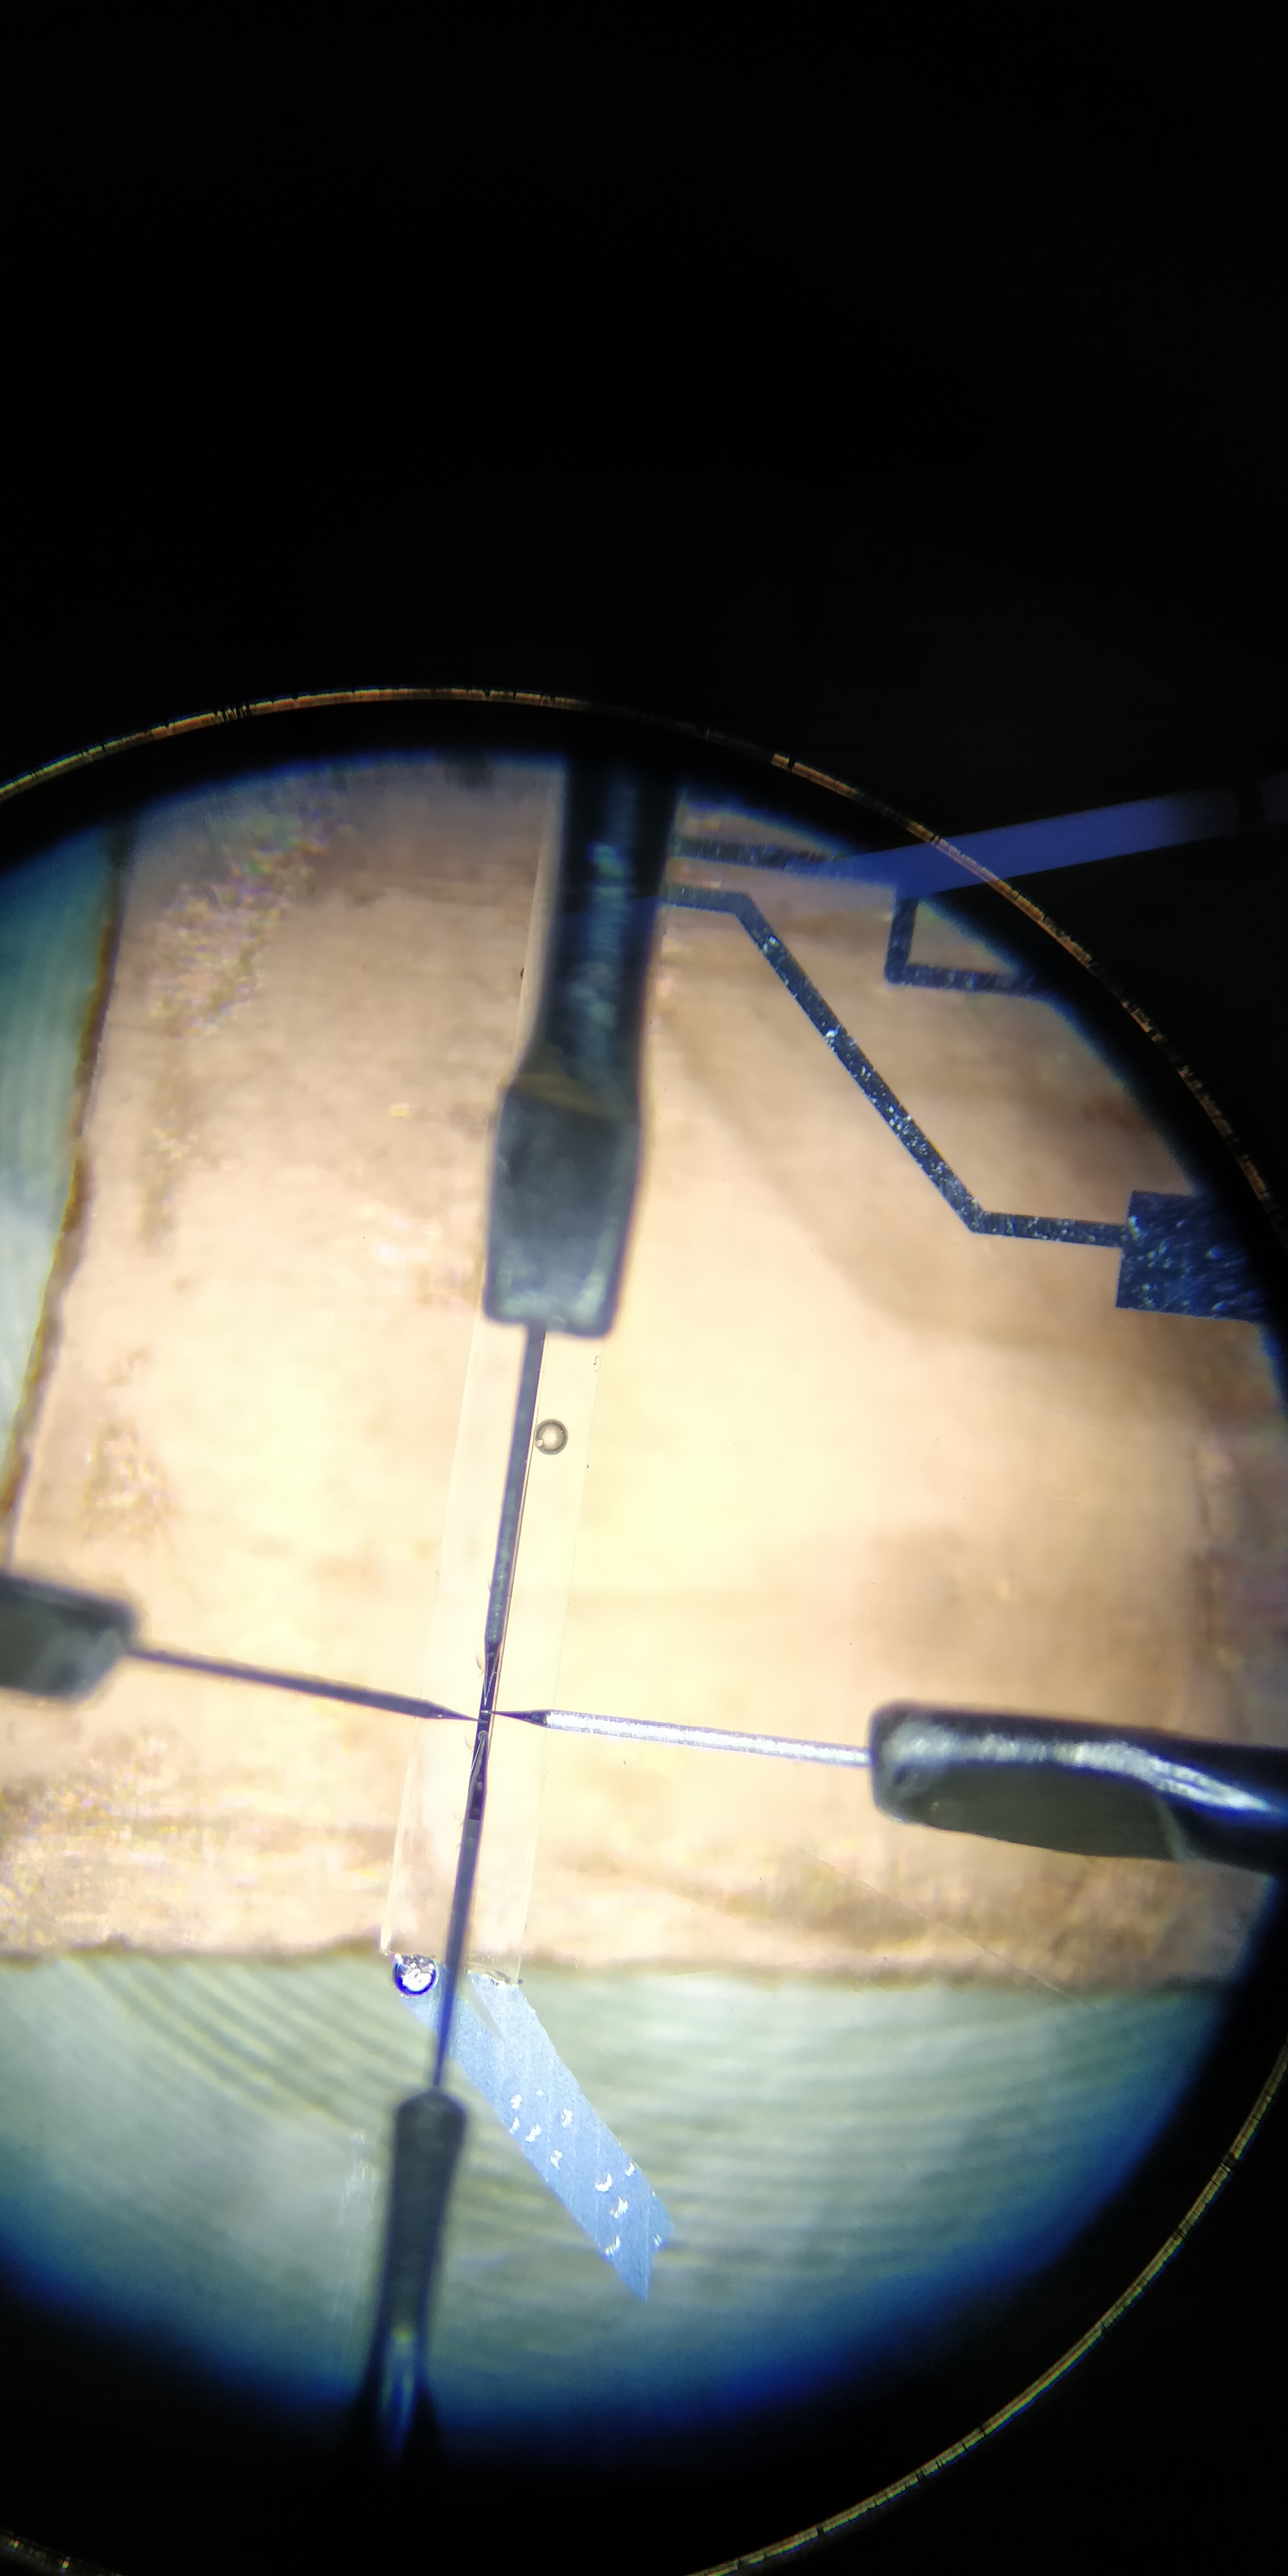
\includegraphics[]{IMG_20190409_143409.png}


\end{document}
